% Chapter Template

\chapter{Results} % Main chapter title

\label{Chapter6} % Change X to a consecutive number; for referencing this chapter elsewhere, use \ref{ChapterX}

%----------------------------------------------------------------------------------------
%	SECTION 1
%----------------------------------------------------------------------------------------

\section{Test Preparation}

\subsection{Hardware}
The CPU used for testing desktop performance is an \textbf{Intel i7 7700HQ} @ 2.80 GHz with 4 cores (8 virtual cores) \cite{intel7700hq}. It is a 7th generation 64-bit Intel processor with SSE, SSE2, SSE3, SSSE3, SSE4\_1, SSE4\_2, AVX and AVX2 extensions. Both 32-bit and 64-bit code was tested on this CPU, compiled using Rust compiler with corresponding targets. The operating system running is Ubuntu 18.10.\\
\\
For testing on mobile devices, we used \textbf{Samsung S9's Exynos} processor. It has 8 cores: 4 cores run at 2.9 GHz, and the other four at 1.9 GHz \cite{exynos9810}. Both 32-bit and 64-bit code was tested on this processor, using corresponding targets for the Rust compiler, and Android NDK (\texttt{armv7a-linux-androideabi16} for 32-bit code, and \texttt{aarch64-linux-android21} for 64-bit code).\\
\\
\textbf{Intel HD Graphics 630} is a GPU integrated with 7700HQ. It has 24 processing units working at a frequency of 350 MHz during normal operation, and 1.1 GHz burst frequency \cite{intelhd630}. It has access to system RAM. NEO Linux drivers were used.\\
\\
\textbf{Mali-G72 MP18} is a GPU integrated with Samsung's Exynos processor on Galaxy S9. It has 18 processing units working at 850 MHz \cite{mali}. It has access to system RAM.\\
\\
\textbf{NVIDIA GTX 1060M 6GB} is a GPU with 1280 computation units working at a frequency of 1404 MHz (1670 MHz boost frequency). It houses 6 GB of global memory. 1280 CUDA cores are divided equally among 10 SMs (streaming microprocessors). Each SM has 256 KB of private memory, 96 KB of shared memory, as well as a 48 KB L1 cache \cite{nvidia1060}. Proprietary NVIDIA Linux drivers were used.\\
\\
\textbf{AMD RX 580} is a GPU with 2304 streaming processors (SP) grouped in 36 Compute Units (CU) operating at 1257 MHz (1340 MHz boost). Every streaming processor has 256 vector registers and 512 scalar registers, each 4 bytes wide (64 KB + 8 KB total). Every compute unit also has 64 KB of shared memory and a complex cache hierarchy \cite{amdrx580}.\\

\section{OpenCL Support on Different GPUs}

Considering that only 6\% of OpenCL papers test the program on 3 or more different platforms \cite{sorensen2016hitchhiker}, we will take this opportunity to list the difficulties we've encountered. For all GPUs we used ocl Rust crate to run OpenCL code.

\subsection{NVIDIA}
\subsubsection{Setup}
NVIDIA driver officially supports only OpenCL 1.2. Recently, there has been some progress towards the more modern standard, with NVIDIA quietly enabling OpenCL 2.0 \cite{nvidiareleasenotes}. NVIDIA has been pushing its GPGPU solution CUDA over OpenCL, and OpenCL is expected to perform slightly slower than equivalent CUDA code \cite{fang2011comprehensive, karimi2010performance}. This is also visible in dropping support for OpenCL code profiling that was present in older driver versions \cite{nvidiaprofiler}. However, we've managed to get static kernel data and assembly by dumping the high-level assembly (PTX file) and compiling it for the architecture that our card supports (Compute Capability 6.1). CUDA occupancy calculator was then used to estimate how many threads' states could be saved at the same time.
\subsubsection{Runtime Bugs}
There was one bug in the compiler that we didn't expect. When compiling a kernel for Four-bit Pippenger, when we loaded only the needed portion of the exponent, we got \texttt{CL\_OUT\_OF\_RESOURCES} error\footnote{It seems that CL\_OUT\_OF\_RESOURCES is treated as a generic error}. The same kernel worked without a problem on Intel's GPU. The error was fixed by reading the entire exponent structure from global memory, instead of only reading the integer that we needed.

\subsection{Intel}
\subsubsection{Setup}
Intel's NEO driver supports OpenCL 2.1. Running longer kernels (more than ~10s) required us to manually disable the watchdog timer in the kernel. Unfortunately, because Intel was the main display device, this caused our device to freeze until kernels finished execution. Due to extremely slow execution speed, we haven't profiled code executing on this GPU.\\\\
\subsubsection{Runtime Bugs}
The biggest issue was encountered when we manually unrolled the square-and-multiply loop (255 iterations). Intel kernel kept outputting the wrong result, but adding \texttt{printf} somehow fixed this problem. NVIDIA GPU outputted the correct result for the same code without any issues. Old Intel driver didn't support \texttt{printf} for 64-bit integers on Ubuntu, but switching to NEO solved this problem. 

\subsection{Mali}
\subsubsection{Setup}
Mali supports OpenCL 2.1. Compiling OpenCL code for Samsung Galaxy S9 required us to dump OpenCL.so from the phone, and link it during compilation. 32-bit code compiled properly even with \texttt{ld} loader, but 64-bit version required us to use \texttt{gold}. It is also interesting that mobile GPUs need low-level ocl crate API (a wrapper around C code). After cross-compiling the binary, which involved some basic symlinking to resolve name conflicts during Rust crate compilation, we used \texttt{adb} and \texttt{adbshell} to copy and run code on the device.\\\\
\subsubsection{Runtime Bugs}
Unfortunately, a compilation of OpenCL kernel results in a \texttt{Segmentation Fault} after a couple of minutes for the 32-bit version. Another problem that we encountered with Mali is the unexpected use of OpenCL API. All other vendors compile the kernel when we call \texttt{clBuildProgram}, while Mali does this during the kernel call. While testing our kernels, we noticed that the application may get killed if the kernel takes too long.

\subsection{AMD}
\subsubsection{Setup}
AMD has the best support for OpenCL of all vendors tested. The only problem we encountered is that profiler GUI wouldn't start, but CLI version had no issues.
\subsubsection{Runtime Bugs}
We haven't encountered any bugs with AMD cards.

\subsection{Conclusion}

OpenCL theoretically enables us to write code only once and run it on different parallel devices. Unfortunately, due to differences in vendors' implementations, it is necessary to test the code on every single device we plan to support. Even then, the code may need to be adapted just to run. Additional debugging is also frequently required, even though code runs properly on other devices. This can pose a problem if the platform provides limited debugging and profiling possibilities (e.g. NVIDIA).

\section{Tests}

\subsection{Whole Proof Generation}

This test involved dumping the data from the actual spending proof generation and running it multiple times on both CPUs with both 32 and 64-bit code. Spending proof has been chosen because it takes longer to generate than the output proof. We also performed a stress test to determine the drop of performance under heavy load.

\begin{figure}[h]
    \centering
    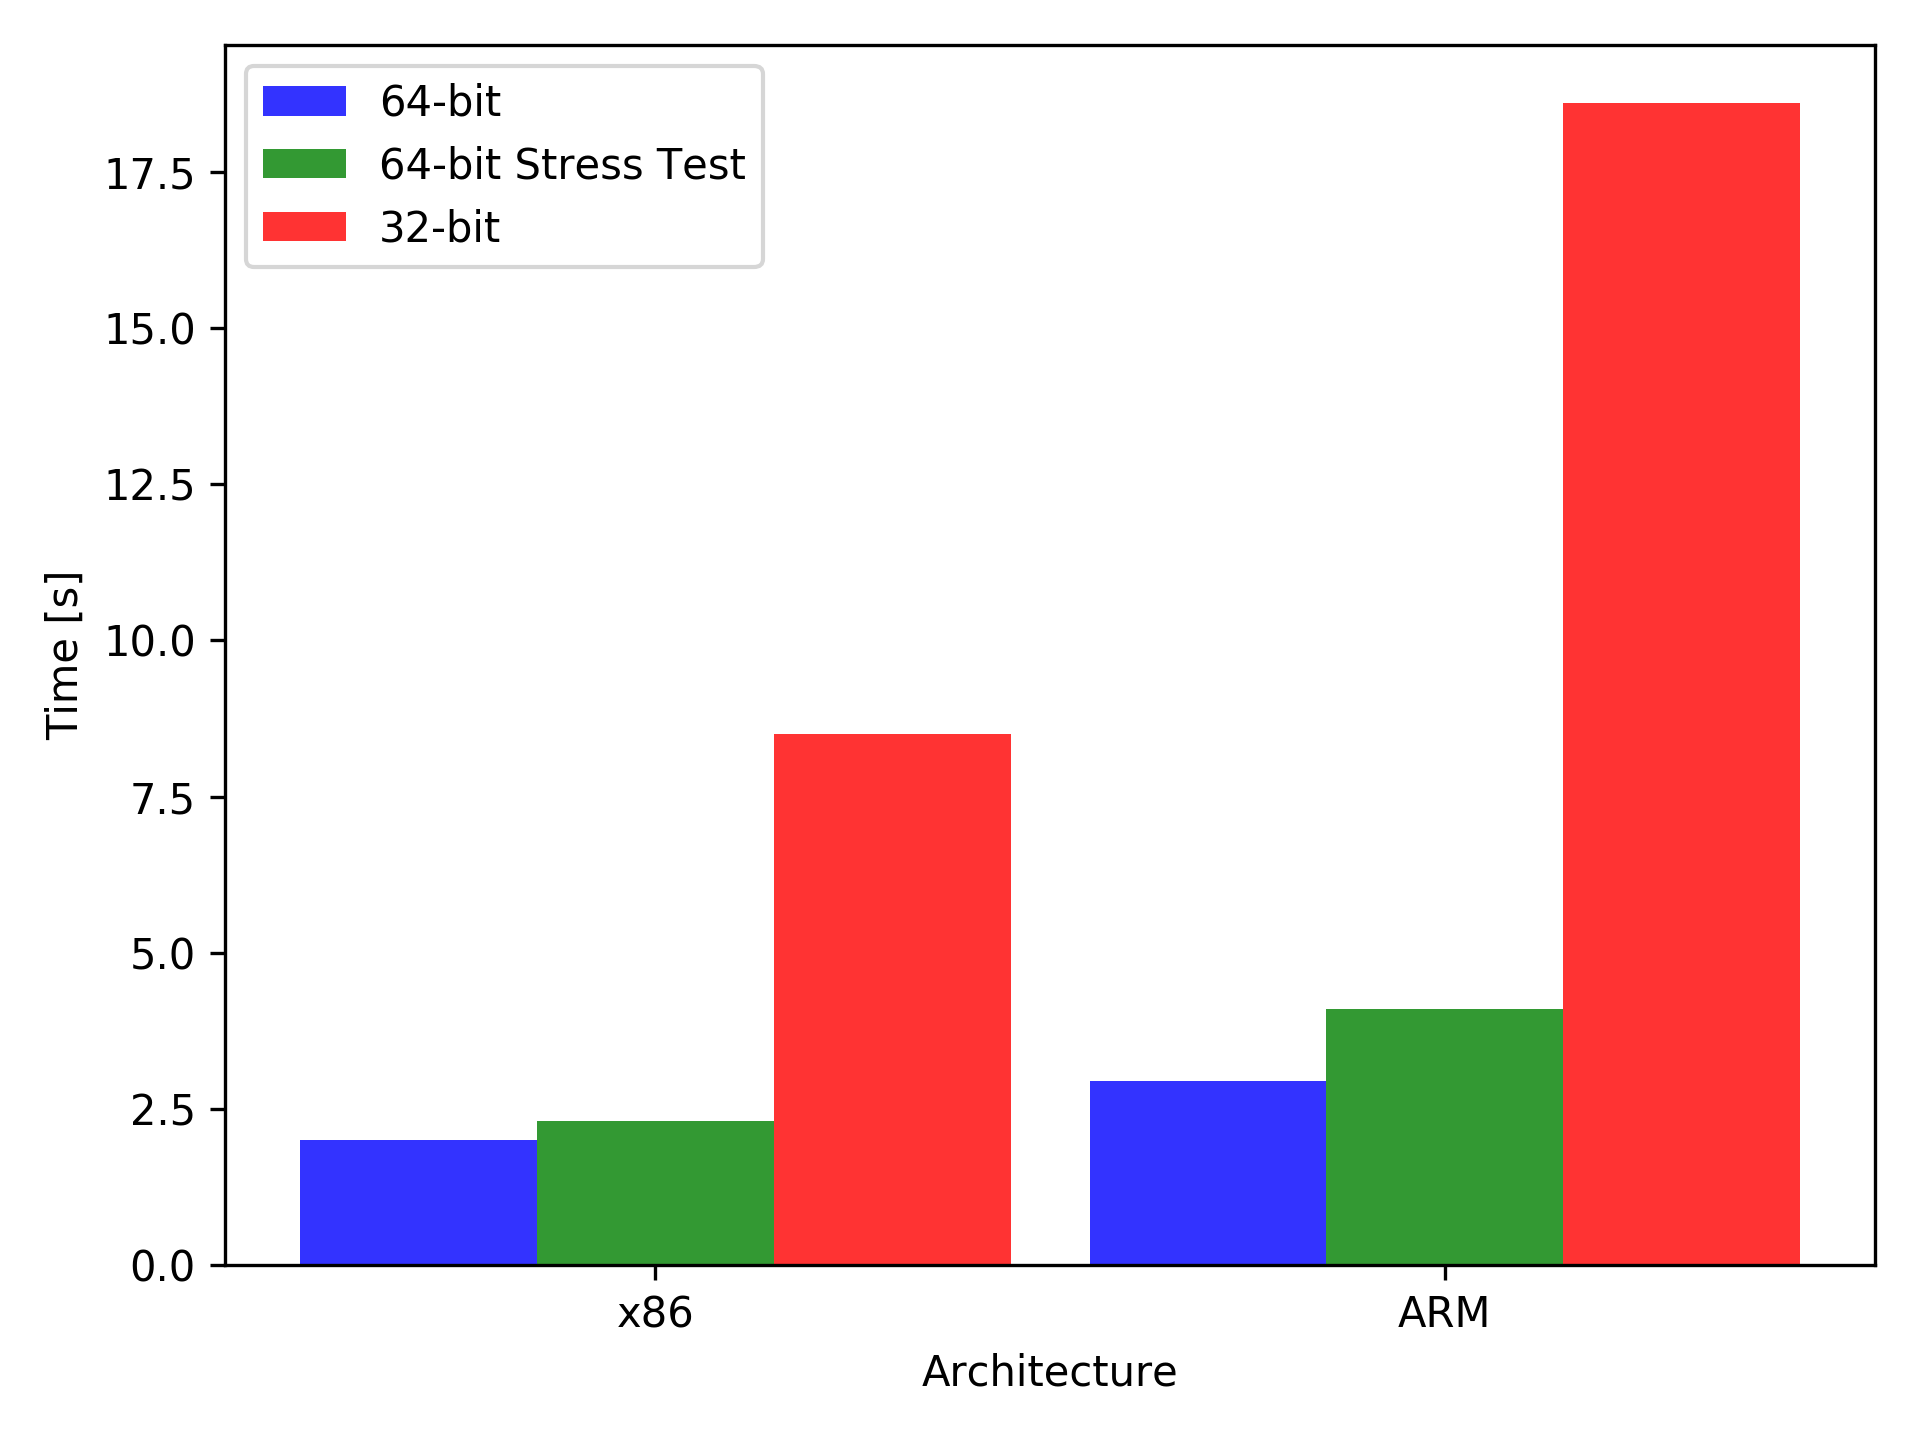
\includegraphics[width=.75\linewidth]{Figures/wholeproof.png}
    \caption{Benchmark of Spending Proof on Various Hardware}
    \label{fig:spendingproof}
\end{figure}

\noindent As we see in Figure \ref{fig:spendingproof}, 32-bit code is significantly slower than 64-bit code. Also, 64-bit ARM code is comparable in performance with x86-64. There is also a slightly larger drop in average performance during the stress test for ARM than for Intel. However, Intel performance was consistent, while the worst-case ARM performance dropped down to 6.75s.

\subsection{FFT and Multiexp}

To determine the best target for optimization we benchmarked different parts of spending proof generation on Intel i7 processor. We benchmarked FFT, Multiexp and witness generation.

\begin{figure}[h]
    \centering
    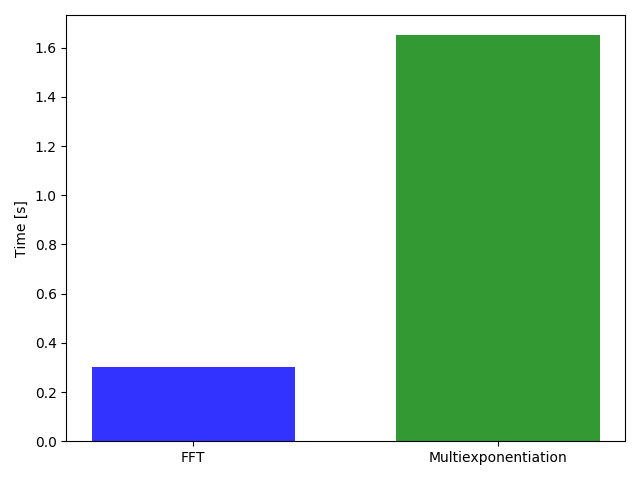
\includegraphics[width=.75\linewidth]{Figures/proofparts.png}
    \caption{Benchmark of FFT and Multiexponentiation in a Spending Proof}
    \label{fig:partsbenchmark}
\end{figure}

\noindent CPU spends the most time performing FFT and multiexponentiation. Witness generation takes several milliseconds at most. In Figure \ref{fig:partsbenchmark} we can see that multiexponentiation takes 85\% time of proof generation. This made multiexponentiation a natural target for optimization. To determine potential for parallelization, we also benchmarked single-core performance and plugged in the numbers into Amdahl's law. This gave us 88.5\% of parallel code (in theory).\\

\subsection{131k Test}

We decided to benchmark our multiexponentiation algorithms on group G1, with ~131k points and exponents. This is the size of the largest array that gets processed. $\mathbb{G}_1$ group was selected because it is simpler to implement and is used more often than $\mathbb{G}_2$.
\begin{figure}[h]
    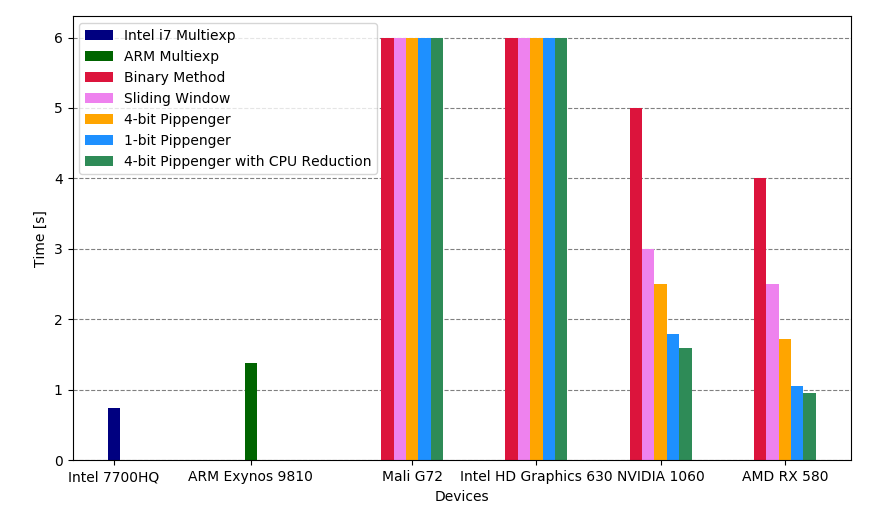
\includegraphics[width=\linewidth]{Figures/finalresults.png}
    \caption{Comparison of Algorithms Implemented Running on Various Hardware}
    \label{fig:finalresults}
\end{figure}
 \noindent The data for integrated GPUs (Intel and Mali) shown in Figure \ref{fig:finalresults} has been cut off at 6 seconds. The actual times are much higher -- several minutes for Mali and 10.4 seconds for the best Intel kernel. NVIDIA and AMD perform better, but still not at the level of CPUs. Square-and-multiply takes the most time, followed by windowed-square-and-multiply. Variants of Pippenger's algorithm are the fastest, with 4-bit Pippenger with CPU reduction taking the first spot. Unfortunately, even it fails to overtake multiexponentiation on Intel i7.
